\documentclass[conference]{configs/IEEEtran}
\IEEEoverridecommandlockouts
% The preceding line is only needed to identify funding in the first footnote. If that is unneeded, please comment it out.
\usepackage{cite}
\usepackage{amsmath,amssymb,amsfonts}
\usepackage{algorithmic}
\usepackage{graphicx}
\usepackage{textcomp}
\usepackage{xcolor}
\usepackage{hyperref}
\def\BibTeX{{\rm B\kern-.05em{\sc i\kern-.025em b}\kern-.08em
    T\kern-.1667em\lower.7ex\hbox{E}\kern-.125emX}}
\begin{document}

\title{Development of Performance Regression Analysis Tool using Distributed Tracing on Microservice-based Application\\
%{\footnotesize \textsuperscript{*}Note: Sub-titles are not captured in Xplore and should not be used}
%\thanks{Identify applicable funding agency here. If none, delete this.}
}

\author{\IEEEauthorblockN{Rafi Abbel Mohammad}
\IEEEauthorblockA{\textit{School of Electrical Engineering and Informatics} \\
\textit{Institut Teknologi Bandung}\\
Bandung, Indonesia \\
masterraf21@gmail.com}
%\and
%\IEEEauthorblockN{Achmad Imam Kistijantoro}
%\IEEEauthorblockA{\textit{School of Electrical Engineering and Informatics} \\
%\textit{ITB, Indonesia}\\
%Bandung, Indonesia \\
%imam@stei.itb.ac.id}
}

\maketitle

\begin{abstract}
In applications with Microservice architecture, when a significant change occurs and result in decreased performance or regression, it is difficult to perform analysis to check which part of the whole Microservice is the main cause of the regression due to the distributed nature of Microservice. Distributed tracing can be used to analyze and determine whether there is a regression and the cause of the regression by utilizing latency data from existing operations on Microservice application.
This system will perform performance regression analysis using the distributed tracing tool Zipkin. Regression is then can be detected using Kolmogorov-Smirnov statistical analysis which will compare the latency data samples that occur
periodically and the sample latency baseline data that represents application performance  under normal circumstances. The analysis will compare the Cummulative
Distribution Function (CDF) of the two samples and see if both
CDF comes from a different distribution. If it is found that both CDFs originate from different distributions, it then can be suspected that there has been a performance regression because the distribution of the periodic data has deviated from the distribution of the baseline data.
If a regression is detected, the system will then perform a critical path analysis to see which operations of each services are most likely contributed to the regression. The analysis will be carried out by finding the difference
latency of periodic and baseline operation data and it will be seen which operation's latency difference exceeds a predetermined limit.
The performance regression analysis system has been tested on a Microservice application that runs on Kubernetes. The result is that out of 10 out of 11 test cases, and for every successful case, the main suspected operation that causes regression is found. Implementing the system adds an average overhead of 0.78\% CPU usage and 0.67\% Memory usage.
\end{abstract}

\begin{IEEEkeywords}
performance regression, Distributed Tracing, Microservice, Kubernetes
\end{IEEEkeywords}

\section{Introduction}
\label{1}
With the widespread adoption use of Microservice architecture based on distributed systems today, more and more challenges arise related to the adoption of this architectural style. Microservice architecture offers several advantages, including technological heterogeneity, resilience, ease of \textit{scaling}, ease of \textit{deployment}, ease of alignment with a technology team, flexibility in determining application composition, and an optimized system to replace components with each other \cite{building-microservices}. These advantages make the adoption of the Microservice architecture quite widespread, especially in applications that require \textit{scalability} to serve the growing needs of customers.

However, with the many advantages offered by the Microservice architecture, it will also increase the complexity to perform analysis when there is a decline in performance or regression in the application. This is due to the distributed nature of Microservice by dividing the application into smaller services, so to find which operation of the services causing the regression will be difficult and will be inefficient to perform analysis on each and every available services, especially if the number of the services has reached hundreds or thousands.

There is already a tool that can help developers to perform monitoring on distributed systems such as Microservice, which is distributed tracing. With the help of trace, developers can get an overview of each request that occurs in a resource or component that interacts with other components in a distributed system such as node, service, network, or mutex. The traces then can be processed for various purposes, such as creating a dependency map between services, perform a performance analysis of the service, and also perform a performance regression analysis using the latency data from the trace result.

We provide the implementation of the performance regression analysis (PRA) system using the distributed tracing tool Zipkin which is available on Github\footnote{\url{https://github.com/masterraf21/pra\textunderscore engine}}. The PRA system will perform detection on the Microservice application when a regression occurs and perform analysis to determine the main cause of the regression. Performance regression analysis will be done by using the help of the trace results from Zipkin which will be able to help developers restore performance of Microservice application after reggresion occurs.

The paper is organized as follows. Section II presents related
work in the area of performance regression and distributed tracing. Section III discusses problem analysis, the design and the underlying architecture, and the implementation of the PRA system. Section IV shows the experiments done with the PRA system. Section V discusses a few analysis from the experiments done in Section V. Section
VI concludes the work.


\section{Related Works}

\section{Proposed Solution}
This section explains analysis of the problem introduced in section \ref{1}, the general solution to solve the problem, the architecture, and the implementation of the system.

\subsection{Problem Analysis}
Fig. \ref{arch-pra} shows the architecture of the PRA system inside a Kubernetes cluster.
\begin{figure}[!htb]
	\centering
	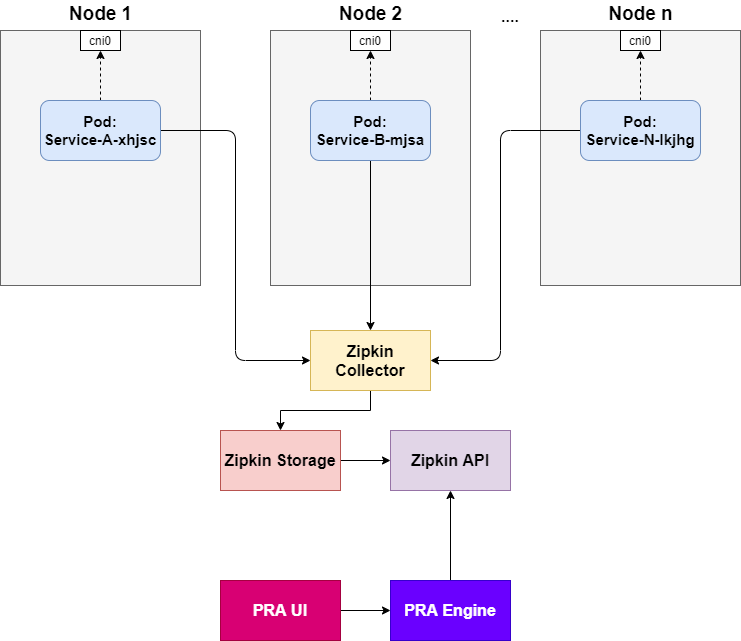
\includegraphics[width=0.5\textwidth]{resources/ch3/arch.png}
	\caption{Arsitektur sistem \textit{Performance Regression Analysis} (PRA)}
	\label{arch-pra}
\end{figure}

\subsection{Architecture}

\subsection{Implementation}

\section{Experiment}

\section{Analysis}

\section{Conclusion \& Future Works}

%\section*{Acknowledgment}
%
%The preferred spelling of the word ``acknowledgment'' in America is without 
%an ``e'' after the ``g''. Avoid the stilted expression ``one of us (R. B. 
%G.) thanks $\ldots$''. Instead, try ``R. B. G. thanks$\ldots$''. Put sponsor 
%acknowledgments in the unnumbered footnote on the first page.

\bibliographystyle{configs/IEEEtran}
\bibliography{references}

\vspace{12pt}


\end{document}
